\section{MOS Transistoren}

\subsection{Dotierung}
\begin{center}
    \begin{tabular}{lll}
        \textbf{Dotierung:}          & N-dotiert            & P-dotiert \\
        \textbf{Unreinheit:}         & Aluminium (HG III)   & Phosphor / Arsen (HG V) \\
        \textbf{Majoritätsträger:}   & Elektronen           & Löcher \\
        \textbf{Minoritätsträger:}   & Löcher               & Elektronen \\
    \end{tabular}
\end{center}

\subsection{MOS-Kondensator}
\begin{minipage}{0.5\columnwidth}
    Minoritätsträger werden an das Gate gezogen.
    Die entstandene Raumladungszone weist bei ausreichend hoher Gate-Spannung einen Minoritätsträgerüberschuss auf, ist also in der Funktion komplementär zum Substrat dotiert.
\end{minipage}
\hfill
\begin{minipage}{0.4\columnwidth}
    % TODO: evtl. klärendes Bild
\end{minipage}

\subsection{MOS-Transistoren}
Werden links und rechts vom MOS-Kondensator komplementär zum Substrat dotierte Regionen (Drain und Source) erstellt, so kann ohne Gatespannung aufgrund der PN-Übergänge kein Strom vom Drain zur Source (oder umgekehrt) fliessen.
Wird nun eine Spannung am Gate angelegt, so entsteht die Minoritätsträger-Leitende Raumladungszone - der Kanal.
Dieser verbindet Drain und Source, es kann also ein Strom fliessen.

\begin{center}
    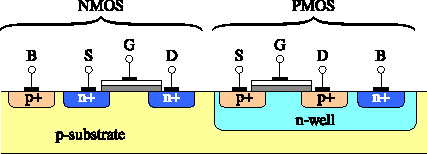
\includegraphics[width=0.5\columnwidth, align=t]{images/01_CMOS.pdf}
\end{center}

\subsubsection{Variationen}
Durch vordotierung des Kanals kann der Transistor ohne Gate-Spannung leitend gemacht werden.
Eine negative Gate-Spannung kann den Kanal dann abschnüren.
Dies ist ein Verarmungs-MOSFET.

% TODO: Tabelle V2 S13

Der Bulk wird nur eingezeichnet, wenn dieser nicht mit der Source verbunden ist.

\subsubsection{Modelle}
In Cadence sind verschiedene Modelle hinterlegt:

\textbf{Berkly Model 11:} Das Modell 11 wurde in Berkly erstellt und beinhaltet eine Vielzahl Parameter und ist recht komplex.

\textbf{Model 1:} Handrechenmodell, welches zwar weniger genau, dafür aber viel einfacher ist.

\subsection{Arbeitsbereiche von MOS-Transistoren}
Der Ausgangsspannungsbereich, also die $V_DS$-Achse wird in zwei Teile unterteilt: Gesättigt und ungesättigt.

Der Ausgangsstrombereich, also die $V_{GS}$-Achse wird in die folgenden Bereiche unterteilt:
\begin{description}
    \item[Leckstrom-Bereich:] Der Transistor leitet aufgrund von parasitären Effekten nur minimal.
    \item[Weak Inversion:] Durch den Kanal beginnt Strom zu fliessen, $I_D$ steigt exponentiell mit $V_{GS}$.
    \item[Moderate Inversion:] Der Übergangsbereich zwischen Weak und Strong Inversion, schlecht mit Formeln modellierbar.
    \item[Strong Inversion:] Der Kanal leitet, $I_D$ steigt quadratisch mit $V_{GS}$.
\end{description}
%TODO: evtl. Kennlinie aus V2 S19

\subsubsection{Sättigung}
% TODO: evtl. Bilder zu den Ladungsträgervertielungen aus V2 S15
Die Sättigungsgrenze ist gegeben als
\[\boxed{V_{DS} > V_{DS\text{, sat}}}.\]

Für Weak Inversion gilt
\[\boxed{V_{DS\text{, sat}} = V_{GS}-V_T}.\]

Moderate und Strong Inversion gilt
\[\boxed{V_{DS\text{, sat}} = 5 \cdot V_\text{temp} \approx \qty{130}{mV}}.\]

\[V_\text{temp} = \frac{kT}{q}\]

$k$: Boltzmann-Konstante

$q$: Elementarladung

$T$: Temperatur in Kelvin


\subsubsection{Leakage affected Region}
\begin{center}
    \[\boxed{V_{GS} < V_K(I_D)}\]
\end{center}

Keine Formel für $I_D$ gegeben.

\subsubsection{Weak Inversion}
\[\boxed{V_K(I_D) < V_{GS} < V_M(I_D)}\]
\[ V_M(I_D) = V_T(I_D) - x_M(I_D) \]
\medskip

\begin{minipage}{0.48\columnwidth}
    Ungesättigt:
    \[I_D = I_M \cdot \e^{\frac{V_{GS} - V_M}{n_M \cdot V_\text{temp}}} \cdot (1 - \e^{-\frac{V_{DS}}{V_\text{temp}}})\]
\end{minipage}
\hfill
\begin{minipage}{0.48\columnwidth}
    Gesättigt:
    \[I_D = I_M \cdot \e^{\frac{V_{GS} - V_M}{n_M \cdot V_\text{temp}}}\]
\end{minipage}

\subsubsection{Moderate Inversion}
\begin{center}
    \[\boxed{V_M(I_D) < V_{GS} < V_H(I_D)}\]
    \[ V_H(I_D) = V_T(I_D) + x_H(I_D) \]
\end{center}

Keine Formel für $I_D$ gegeben.

\subsubsection{Strong Inversion}
\begin{center}
    \[\boxed{V_H(I_D) < V_{GS} < V_L(I_D)}\]
\end{center}

\medskip

\begin{minipage}{0.48\columnwidth}
    Ungesättigt:
    \[I_D = \mu C_{\text{OX}} \cdot \frac{W}{L} ((V_{GS} - V_T) V_{DS} - \frac{[V_{DS}^2]}{2})\]
\end{minipage}
\hfill
\begin{minipage}{0.48\columnwidth}
    Gesättigt:
    \[I_D = \frac{\mu C_{\text{OX}}}{2} \cdot \frac{W}{L} (V_{GS} - V_T)^2\]
\end{minipage}

\subsubsection{Linear Region}
\begin{center}
    \[\boxed{V_L(I_D) < V_{GS}}\]
\end{center}

Keine Formel für $I_D$ gegeben.

\subsection{Kennlinien}
% TODO: Datenblattauszug (Kennlinie) aus V2 S14 oder S15
% TODO: 3D - Kennlinie aus V2 S21

\subsection{Ersatzschaltungen}
% TODO: Bilder der Ersatzschaltungen

\subsubsection{Gesättigt}
\begin{center}
    \[\boxed{I_D = f(V_{GS})}\]
\end{center}

\subsection{Ungesättigt}
\begin{center}
    \[\boxed{I_D = f(V_{DS})}\]
\end{center}